\chapter{Growing a Social Page as a Distribution System}

This chapter follows a School of Hard Knocks entrepreneurship lesson, curated by LazyingArt LLC through Video2Book, on growing Instagram and Facebook pages. The lecture is practical rather than theoretical: it begins from the speaker's four years in digital marketing, then turns that experience into a sequence of operating rules. We will keep the order of that sequence. The central idea is that page growth is not one trick but a feedback system: post consistently, find a repeatable content supply, choose formats with organic reach, give the algorithm relevant signals, remove platform friction, and keep testing.

\section{The Claim: Growth Becomes Repeatable}

The speaker opens by saying that he has been in digital marketing for about four years, working across social media pages and channels. In that time he has grown pages consistently, but only recently, over roughly the previous six months, has he noticed a few ingredients that behave like a formula for faster growth.

The word ``formula'' should not be read as a guaranteed equation. It is closer to an operating model. A page grows when several conditions are kept active at once:
\begin{equation}
\text{Growth system}
=
\text{cadence}
+
\text{content supply}
+
\text{distribution format}
+
\text{audience signal}
+
\text{feedback}.
\end{equation}

The lecture then proceeds in that order. First we need a cadence. Then we need enough material to support that cadence. Then we need formats and signals that let the platform show the content beyond the existing audience.

\section{Consistency as Momentum Preservation}

The first tip is consistency, and the speaker calls it the most important because it is the foundation for the rest. Once a page has some momentum, the job is not merely to publish occasionally; the job is to keep the page present in the follower's attention.

The practical cadence is stated simply:
\begin{equation}
\text{posting cadence} \in
\{\text{daily},\ \text{every other day}\}.
\end{equation}

This is not presented as a decorative habit. It is the condition that keeps ``top of mind'' awareness alive and keeps loyal followers engaged. In operational terms, consistency is the difference between a page that asks the platform to remember it once in a while and a page that keeps producing fresh engagement signals.

A useful way to write the underlying update rule is:
\begin{equation}
M_{n+1}
=
\alpha M_n + E_n,
\qquad 0 < \alpha < 1.
\end{equation}
Here $M_n$ is the page's current momentum at posting cycle $n$, and $E_n$ is the engagement produced by the next post. The lecture does not write this equation, but it captures the spoken mechanism: if new posts stop arriving, the existing momentum decays; if posts arrive regularly, fresh engagement can replenish it.

\section{Solving the Content Supply Problem}

Once consistency is established, the next obstacle appears immediately. If we are supposed to post daily or every other day, where does the material come from?

The speaker's first answer is to look outward. Visit competitors and pages in a similar space. Look at relevant hashtags. Notice what is trending, what top posts are doing, and what can be adapted to one's own audience. This is not meant as blind copying. It is market observation.

\subsection{Question \& Answer}

\paragraph{Question.}
How do we find enough content without simply stealing from other pages?

\paragraph{Answer.}
The lecture answers with a boundary: use similar pages for inspiration, but give credit when reusing a concrete item. The example is an inspirational Elon Musk quote. If the speaker wants to share it with his own audience, he reposts it and credits the source in the description. That creates a two-sided exchange: his page gets usable content, and the original page gets exposure to another audience.

The same principle applies to Google and image search. We may search an industry plus ``content ideas,'' review long lists of suggestions, and look at old examples. But the output should be adapted to the page, not pasted without context.

The speaker then gives a compact classification of why people look at posts:
\begin{equation}
\text{content demand}
=
\{\text{education},\ \text{entertainment}\}.
\end{equation}
This split matters because it turns content creation into a feedback loop. We do not have to guess forever. We inspect prior analytics, see what worked, see what did not, and model the winning patterns.

\begin{align}
\text{post} &\longrightarrow \text{measure response},\\
\text{measure response} &\longrightarrow \text{identify what worked},\\
\text{identify what worked} &\longrightarrow \text{model and replicate}.
\end{align}

That loop is the bridge from content supply to distribution. A page does not just need more posts; it needs more posts of the kind its audience and platform already show signs of rewarding.

\section{Reels as Organic Distribution}

The second major tip is to use reels. The speaker presents reels as the best way to get large organic reach on Instagram and Facebook, and he emphasizes that the mechanism does not depend only on existing audience size. A page can have five followers or five hundred thousand followers; short-form video still has the possibility of being pushed outward by the platform.

The key comparison is between a static post and a reel:
\begin{equation}
\text{potential reach of reel}
>
\text{potential reach of static post}.
\end{equation}
That inequality is not a universal law, but it is the lecture's practical claim. Reels are treated as a format with more distribution surface.

The speaker then points to TikTok as a source of ideas because short-form creators there have refined the form. The transcript is garbled for a few seconds in this passage, but the intended point is clear enough: if we are making Instagram and Facebook reels, we are already making a kind of content that can also fit TikTok. The same short-form asset can be reused across platforms when it fits the audience.

A concrete threshold appears here:
\begin{equation}
F_{\text{TikTok monetization}} = 10{,}000\ \text{followers}.
\end{equation}
The speaker presents this as a practical monetization milestone, not as the core of the strategy. The core is still distribution: short-form video travels more easily than many static posts.

\section{Hashtags as Audience Routing}

The third tip is that hashtags matter, especially when a page is still getting off the ground. The speaker gives two working counts:
\begin{align}
H_{\text{static post}} &\approx 8\text{--}10,\\
H_{\text{video/reel}} &\approx 6.
\end{align}

The important word is ``relevant.'' A hashtag should describe the actual post or video. The speaker's example is an investing hashtag. If a post tagged with investing starts to get traction, the platform can notice that people who tend to like investing posts are also liking this post. That gives the algorithm an audience signal.

\subsection{Question \& Answer}

\paragraph{Question.}
Why do relevant hashtags matter if the platform is already recommending content?

\paragraph{Answer.}
They matter because they can help route the content. In the lecture's explanation, a relevant hashtag does two things. First, it can help push a post onto the Explore page for people associated with that topic. Second, it can help push the photo or video onto the home feeds of people who do not already follow the page. The hashtag is not magic; it is a signal that helps match the post to a demographic.

\begin{figure}
\centering

\includegraphics[width=\linewidth]{lecture_176_figure_02.png}
\caption{Reel and post insights used to illustrate reach beyond current followers.}
\end{figure}

The frame preserves the analytics context: a Reel Insights panel on the left and a Post Insights panel on the right. The clearest visible Post Insights values are:
\begin{align}
R_{\text{post}} &= 23{,}424,\\
R_{\text{followers}} &= 17{,}478,\\
R_{\text{non-followers}} &= 5{,}946.
\end{align}

From the visible values we can compute the non-follower share:
\begin{align}
\frac{R_{\text{non-followers}}}{R_{\text{post}}}
&=
\frac{5{,}946}{23{,}424} \\
&\approx 0.254.
\end{align}
So, in this visible example, about one quarter of the reached accounts were non-followers. This percentage is a reconstruction from the screenshot, not a number spoken in the lecture.

The same mechanism can be drawn narrowly enough for a pocket layout:
\begin{figure}
\centering
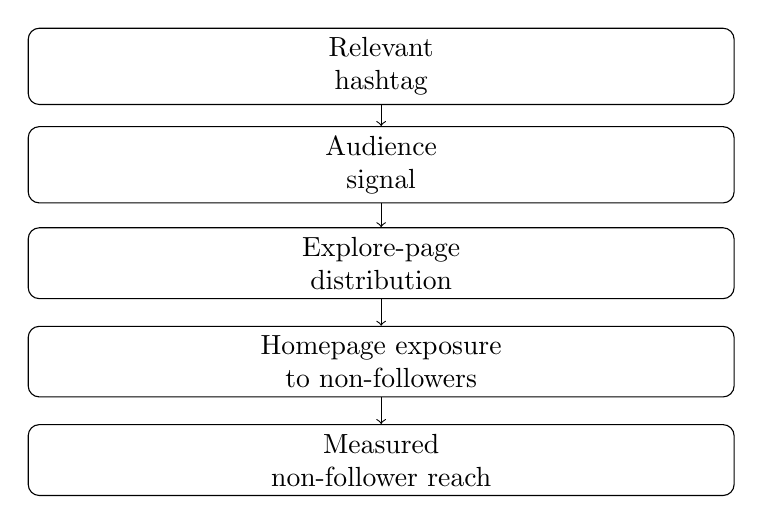
\begin{tikzpicture}
\node[draw, rounded corners, align=center, text width=0.72\linewidth] (a) at (0,0) {Relevant\\hashtag};
\node[draw, rounded corners, align=center, text width=0.72\linewidth] (b) at (0,-1.25) {Audience\\signal};
\node[draw, rounded corners, align=center, text width=0.72\linewidth] (c) at (0,-2.50) {Explore-page\\distribution};
\node[draw, rounded corners, align=center, text width=0.72\linewidth] (d) at (0,-3.75) {Homepage exposure\\to non-followers};
\node[draw, rounded corners, align=center, text width=0.72\linewidth] (e) at (0,-5.00) {Measured\\non-follower reach};

\draw[->] (a) -- (b);
\draw[->] (b) -- (c);
\draw[->] (c) -- (d);
\draw[->] (d) -- (e);
\end{tikzpicture}
\caption{The hashtag mechanism as audience routing rather than decoration.}
\end{figure}

The analytics frame also shows impressions and traffic sources. The clearest right-panel values read approximately:
\begin{align}
\text{Impressions} &\approx 23{,}749,\\
\text{From Home} &\approx 17{,}415,\\
\text{From Explore} &\approx 5{,}283,\\
\text{From Profile} &= 795,\\
\text{From Other} &= 79.
\end{align}
These should be used cautiously because the small screen text is not equally sharp throughout.

\begin{table}
\centering
\begin{tabular}{ll}
\hline
Metric & Visible value \\
\hline
Post accounts reached & $23{,}424$ \\
Followers reached & $17{,}478$ \\
Non-followers reached & $5{,}946$ \\
Non-follower share & $\approx 25.4\%$ \\
Static-post hashtags & $8\text{--}10$ \\
Video/reel hashtags & $\approx 6$ \\
\hline
\end{tabular}
\caption{Compact metric bank for the hashtag and reach discussion.}
\end{table}

The lesson is not simply ``add hashtags.'' The lesson is:
\begin{equation}
\text{relevance} + \text{engagement}
\longrightarrow
\text{better audience routing}.
\end{equation}
If the hashtags are not relevant, the post may not be pushed far. The speaker explicitly adds the patience warning: hashtags may not feel useful at the beginning, but he treats them as one of the key factors in growth.

\section{Friction, Limits, and Calls to Action}

After hashtags, the lecture shifts from distribution signals to operational friction. The next warning is about watermarked videos. The speaker says Instagram and Facebook do not seem to like TikTok-logo watermarks on uploaded videos. His practical observation is that reach improved when he downloaded videos without the watermark before posting.

We can write this as a simple before-and-after claim:
\begin{equation}
\text{reach without watermark}
>
\text{reach with TikTok watermark},
\end{equation}
with an important caveat: this is the speaker's observed platform behavior, not a controlled experiment.

The next growth lever is specific to Facebook. If someone likes a video or photo, the page owner can go to the post reactions and invite that person to like the page. The stated working range is:
\begin{equation}
I_{\text{Facebook invites}} \approx 200\text{--}300
\quad \text{people per batch}.
\end{equation}
The caution is equally concrete:
\begin{equation}
T_{\text{invite ban}} \approx 48\ \text{hours}.
\end{equation}
The speaker says he was banned from inviting people for about that long after doing too much. The point is not fear; it is respecting platform limits.

Finally, the lecture turns to descriptions and calls to action. For static posts, the speaker likes questions: What are your thoughts? What are your opinions? What would you choose? For videos, he likes follower prompts such as ``follow to join the team'' or ``follow to join the movement.'' The description becomes another part of the system:
\begin{equation}
\text{description}
\longrightarrow
\text{comments, follows, watch time}.
\end{equation}

\section{Testing as the Final Operating Rule}

The closing move is experimentation. Try new ideas. Try new tactics. Keep what grows the page. In this lecture, growth is not a single hidden trick but an iterative procedure:
\begin{enumerate}
\item Post consistently.
\item Observe competitors, adjacent pages, and relevant search results.
\item Credit reused material and adapt ideas to the page.
\item Prefer formats, especially reels, with stronger organic distribution.
\item Use relevant hashtags as audience-routing signals.
\item Remove friction such as watermarks.
\item Invite reachable prospects within platform limits.
\item Prompt engagement and follows in descriptions.
\item Read the analytics and repeat.
\end{enumerate}

This is the entrepreneurial payload. The speaker is not separating creativity from measurement. Creativity supplies variants; analytics selects among them. A useful compact form is:
\begin{equation}
\text{growth}
=
\text{creative trials}
+
\text{measured feedback}
+
\text{disciplined repetition}.
\end{equation}

\section{Summary}

The lecture begins with a promise of a growth formula and then builds it in practical order. Consistency preserves momentum. Competitor research, search, credit-based reuse, and analytics solve the content-supply problem. Reels add organic distribution. Relevant hashtags help route content toward the right audience and can produce non-follower reach, as the analytics frame illustrates. Watermarks, invite limits, and calls to action remind us that platform growth is operational as much as creative.

The strongest version of the lesson is not ``post more'' or ``use hashtags.'' It is a measured loop: create, publish, route, observe, and repeat.